%! Author = ryan
%! Date = 12/25/21

% Preamble
\documentclass[11pt]{article}


% Packages
\usepackage{amsmath}
\usepackage[a4paper, total={6in, 8in}]{geometry}
\usepackage{caption}
\usepackage{graphicx}

\title{Ising Simulations}
\author{Ryan T. Grimm}

% Document
\begin{document}

    \maketitle

\begin{abstract}
This document outlines a basic implementation of the two-dimensional Ising model coupled with a Metropolis Monte Carlo.
Initial results of the model show agreement with curves from literature, including heat capacity, magnetization, and magnetic susceptibility,
for a temperature sweep through a phase-transition with zero-field.
\end{abstract}


\section*{Binary Ising}
    We write the Hamiltonian of a two-dimensional ($N \times N$) spin-lattice with spins of $\sigma_{i}$ at site $i$ as
    \begin{align*}
        H _{\{\sigma_i\}}= \sum_{\langle i,j \rangle} J_{i,j} \sigma_i \sigma_j + \sum_i B_i \sigma_i,
    \end{align*} where $\langle i,j \rangle$ represent nearest neighbor pairs, $J$ is the coupling between sites, and $B$ is an external field.
    For this model, we assume that the field and couplings are uniform through the lattice.
    \begin{align*}
        H = J \sum_{\langle i,j \rangle} \sigma_i \sigma_j + B \sum_i \sigma_i,
    \end{align*}
    Additionally, we assume periodic boundary condition.

    The partition function in the canonical ensemble follows from the Hamiltonian.
    \begin{align*}
        Z = \sum_k \exp{\left(-\beta H_{\{\sigma_i\}}\right)}
    \end{align*}


    However, the system size grows like $2^{N \times N}$, which prohibits direct evaluation for non-trivial systems size.
    Thus, we employ Metropolis Monte Carlo to approximate a full enumeration of the configuration space of the lattice.
\section*{Metropolis}
The metropolis algorithm performs a random walk through configuration space while preserving detailed balance and Boltzmann distributed micro-states.
The outline of the algorithm is as follows.
    \begin{enumerate}
        \item Choose a random site $i$.
        \item Compute the change in energy, $\Delta E$, of site $i$ before and after a spin flip.
        \item If $\Delta E \leq 0$, accept the change.
        \item Otherwise, $\Delta E > 0$, accept the change with the probability $P = \exp(- \beta  \Delta E).$
    \end{enumerate} \\


    \begin{figure}
        \centering
        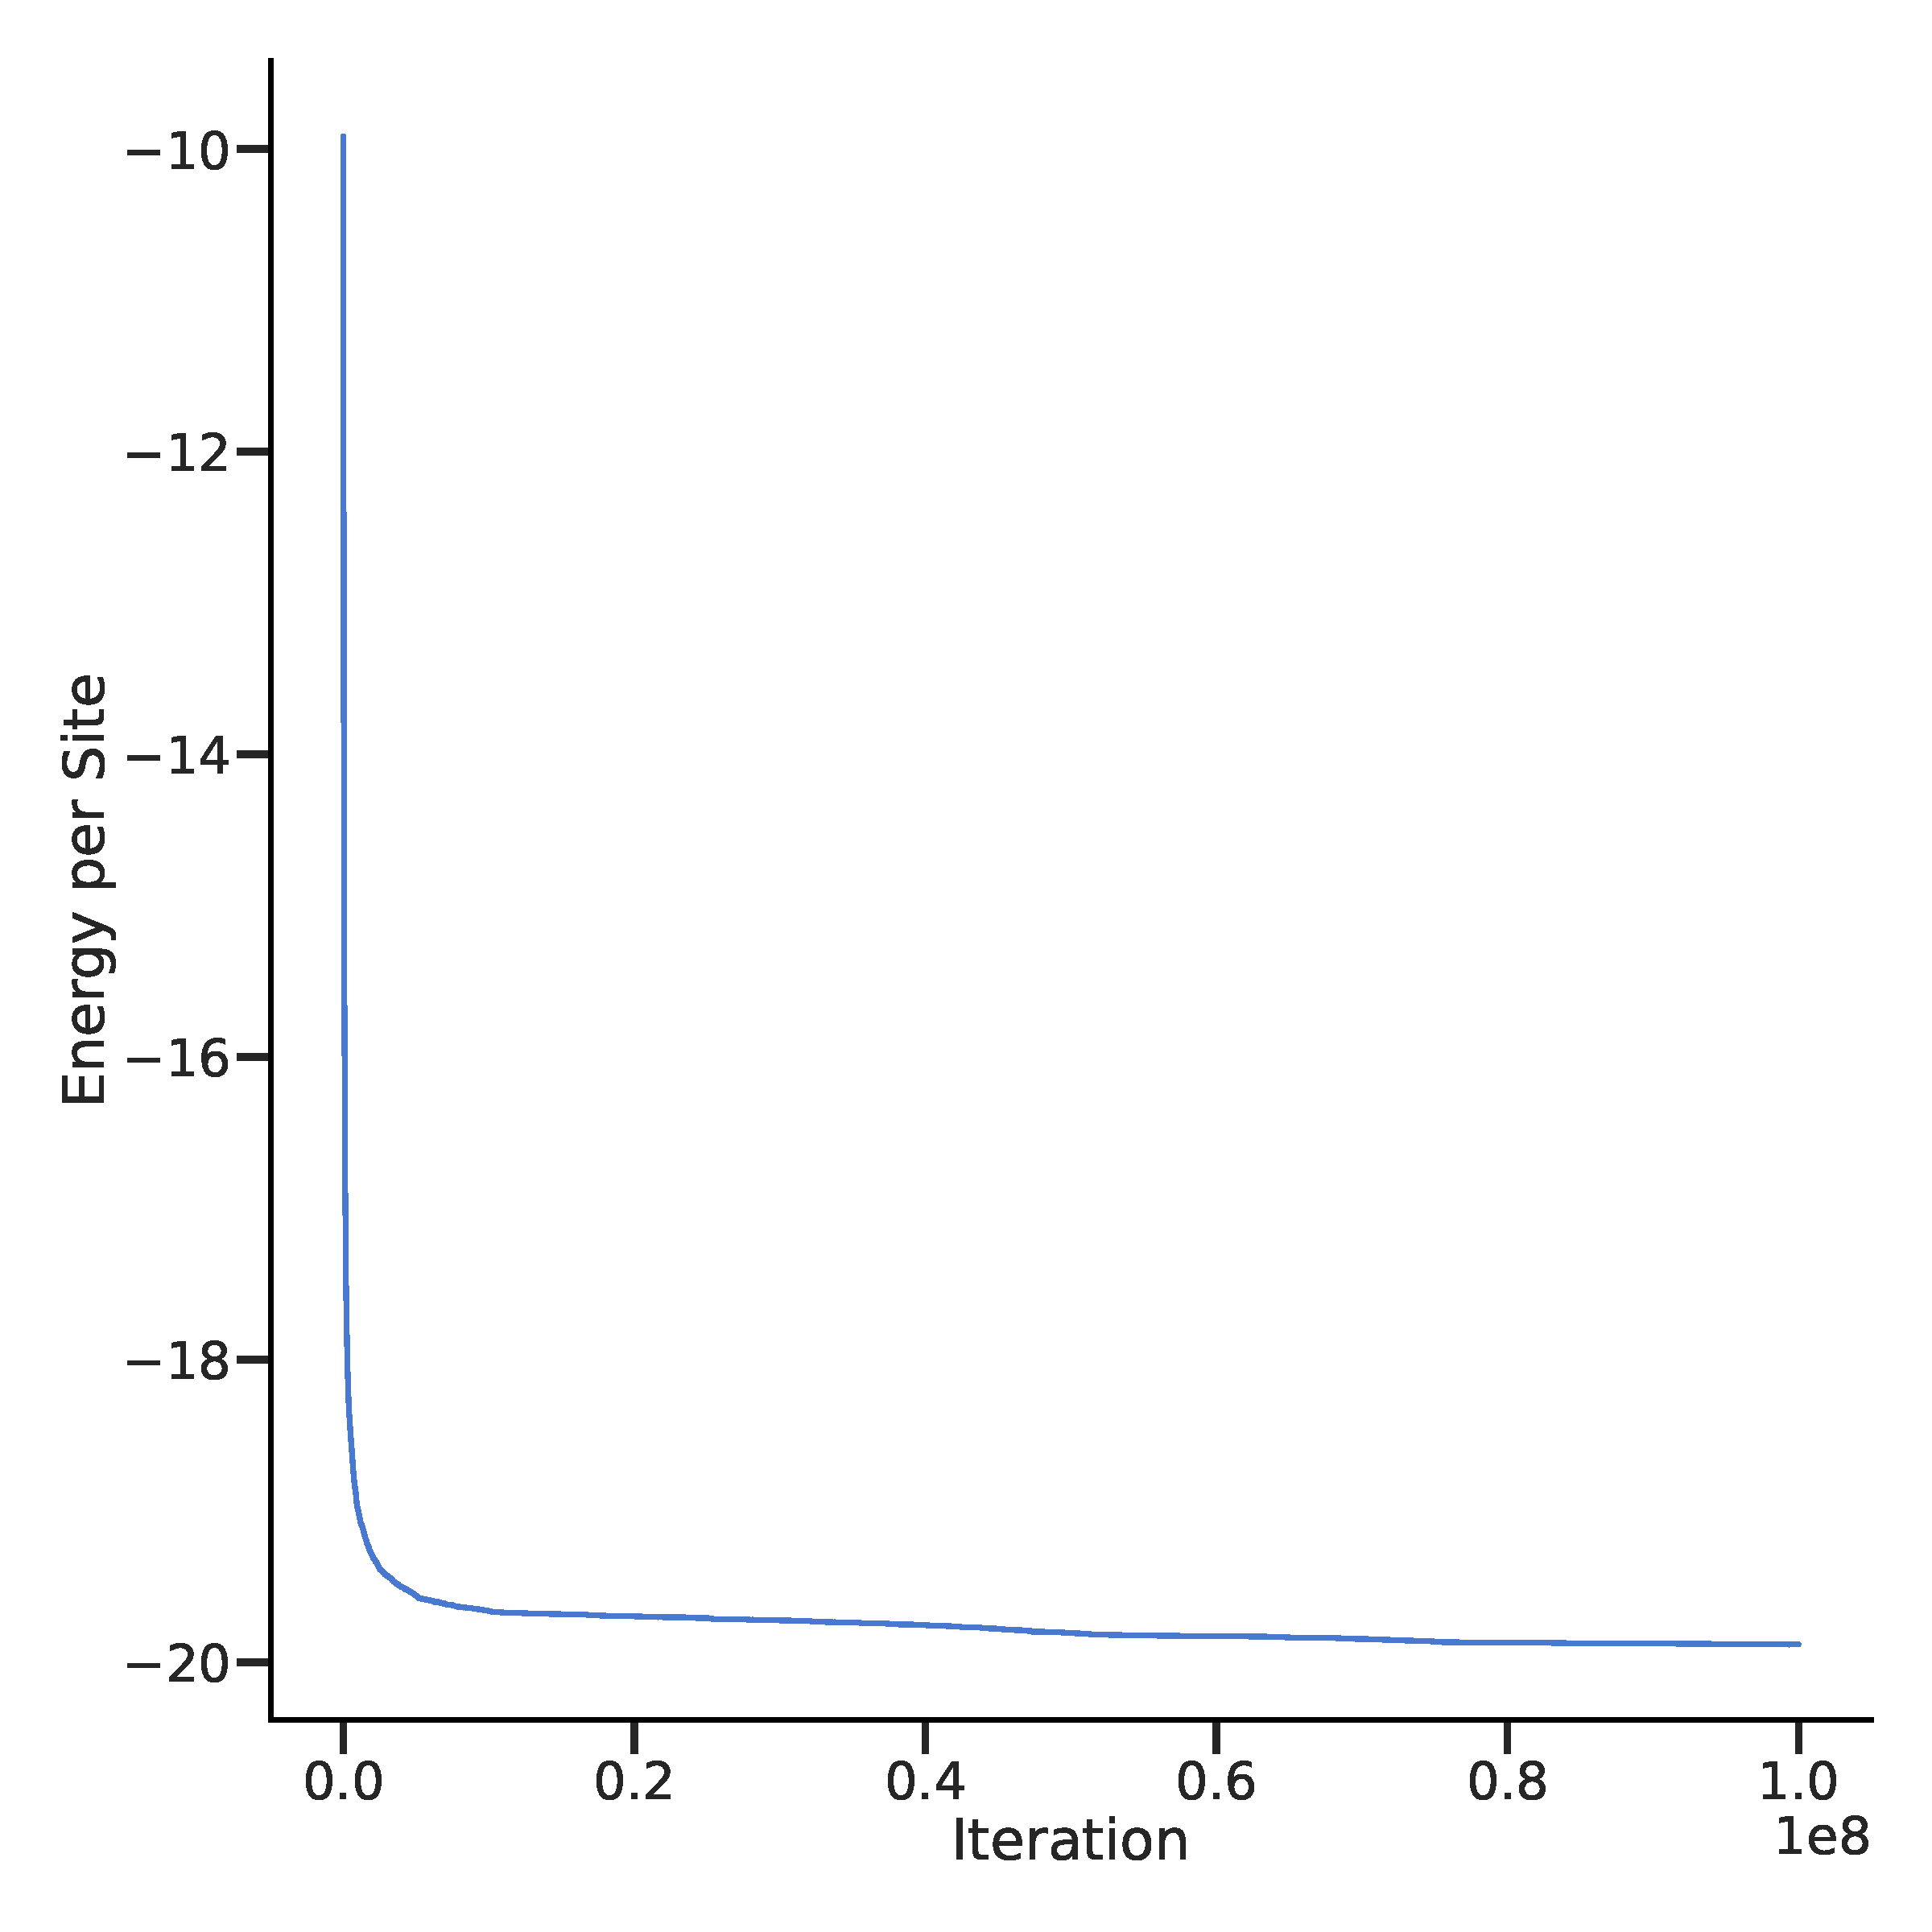
\includegraphics[width=0.6\textwidth]{../Python/eq.pdf}

        \caption{Equilibration of a $128 \times 128$ lattice. }
        \label{fig:eq}
    \end{figure}

First, the algorithm is run to attain an equilibrium configuration of the spin-lattice.
A sampling of a system's micro-states and fluctuations about equilibrium can then be obtained
by running Metropolis on the equilibrium configuration (Figure \ref{fig:eq}).



\end{document}